\section{Hydraulic actuator}

\subsection{Introduction}

  The hydraulic actuators are used to the amplification of the pilot forces. They consist on an actuator body, a input lever, a lever arm and a ram. 
  % -> Components
  % -> Mechanical feedback
  % -> Picture
  % The actuators have different degrees of freedom.

  \begin{figure}[!htpb]
    \centering
    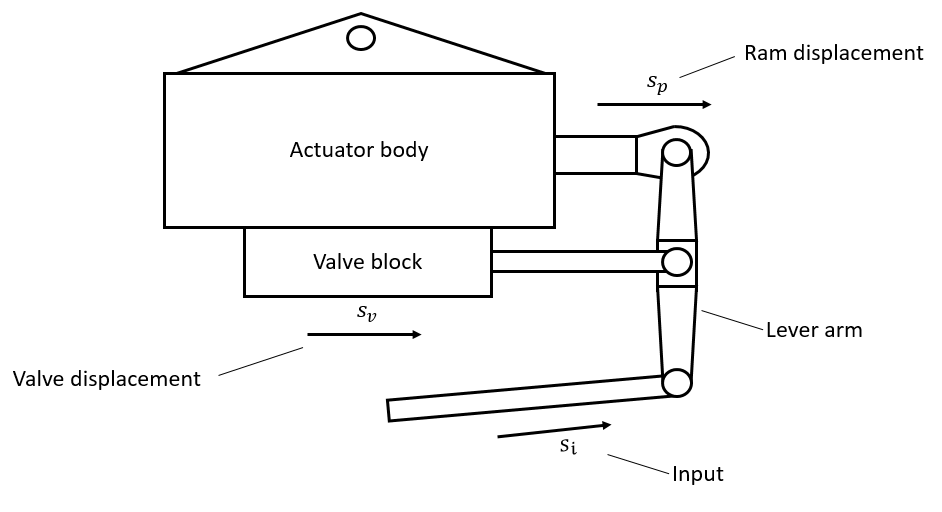
\includegraphics[width=0.7 \textwidth]{figures/diagramActuator}
    \caption[Actuator schematic view]{Actuator schematic view.}
    \label{fig:diagramActuator}
  \end{figure}

\subsection{Modeling}

  The model of a hydraulic actuator is as shown in Figure \ref{fig:modelActuator}. In this model, the internal dynamics of the actuator are represented in terms of force-producer system plus which is mixed with the inertial forces due to the upper controls displacement and the external forces introduced to the aerodynamic surfaces.

  On the left side of the diagram, the pilot input position $x_i$ is mixed to the piston position $x_p$ within the Kinematic lever model. From there, a spool position is extracted and the consequent pressure gain in each of the chambers of the actuator are calculated. The time delay for the spool operation is accounted for with 1st order system block with $T_v$ as time constant. The pressure of the hydraulic fluid acting in each of the piston area $A_{\mathrm{piston}}$ produces a consequent force due to hydraulic pressure $F_{\mathrm{hyd}}$. At this point, the total force acting on the piston rod is calculated adding $F_{\mathrm{hyd}}$ the force due to the Coulomb friction force $F_{\mathrm{f}}$, the force due to the hydraulic damping which opposes the movement of the piston $F_{\mathrm{d}}$ and the force $F_{\mathrm{up}}$ which comes from the inertial forces due to the acceleration of the upper controls components $F_{\mathrm{inertia}}$ and external forces excitation $F_{\mathrm{ext}}$. 

  \begin{figure}[!htpb]
    \centering
    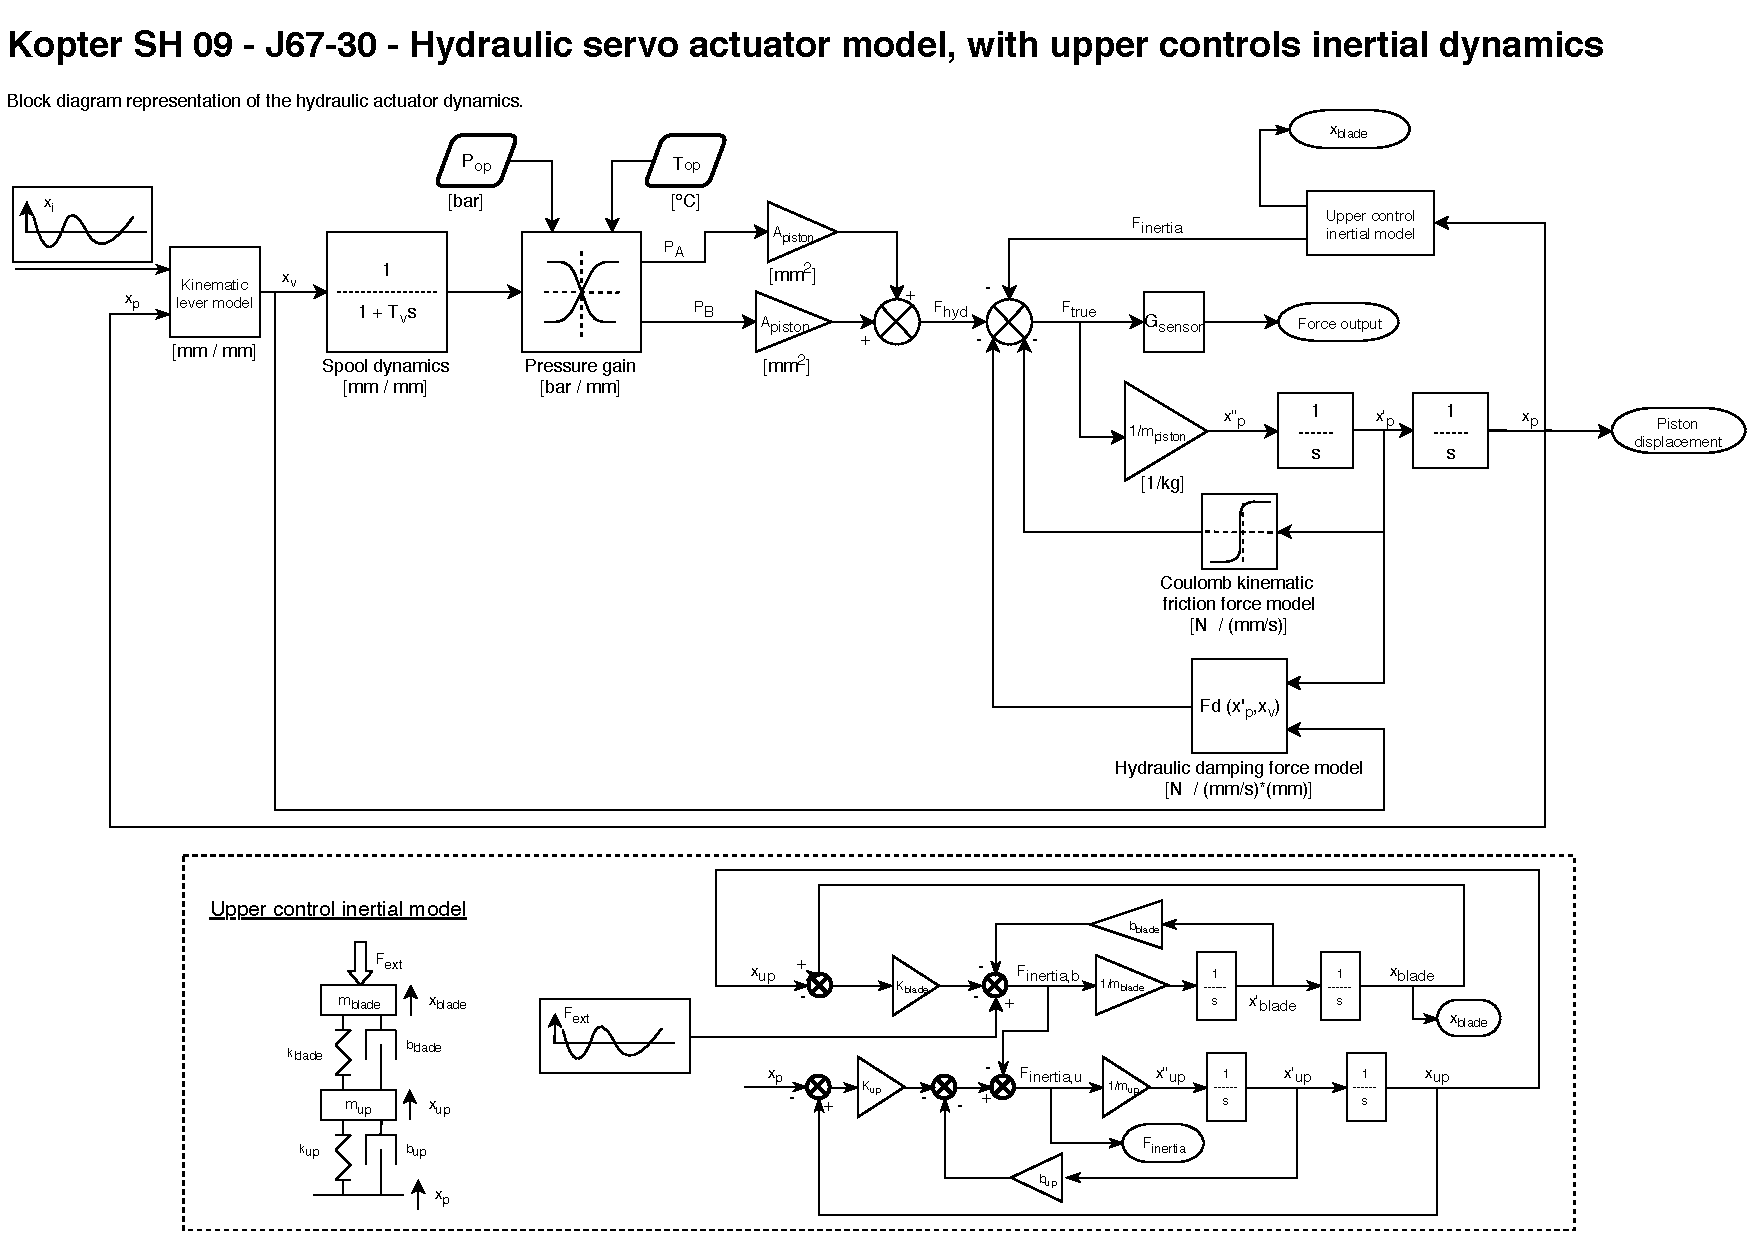
\includegraphics[width=0.9 \textwidth]{figures/modelActuator}
    \caption[Dynamic block model of the hydraulic actuator]{Kopter SH09 Hydraulic servo actuator dynamic block model, with upper controls inertial dynamics and external excitation.}
    \label{fig:modelActuator}
  \end{figure}

  \subsubsection{Pressure gain}

    The name pressure gain is assigned to the relationship between spool position and pressure in each of the four chambers of the hydraulic actuator. This is a nonlinear relationship and it may be different for each system.

    Once the pressure gain curve is obtained, it can be convinient to multiply the obtained pressure by the effective piston area $A_{\mathrm{piston}}$ to arrive to the force gain curve, which is shown in 

    \begin{figure}[!htpb]
      \centering
      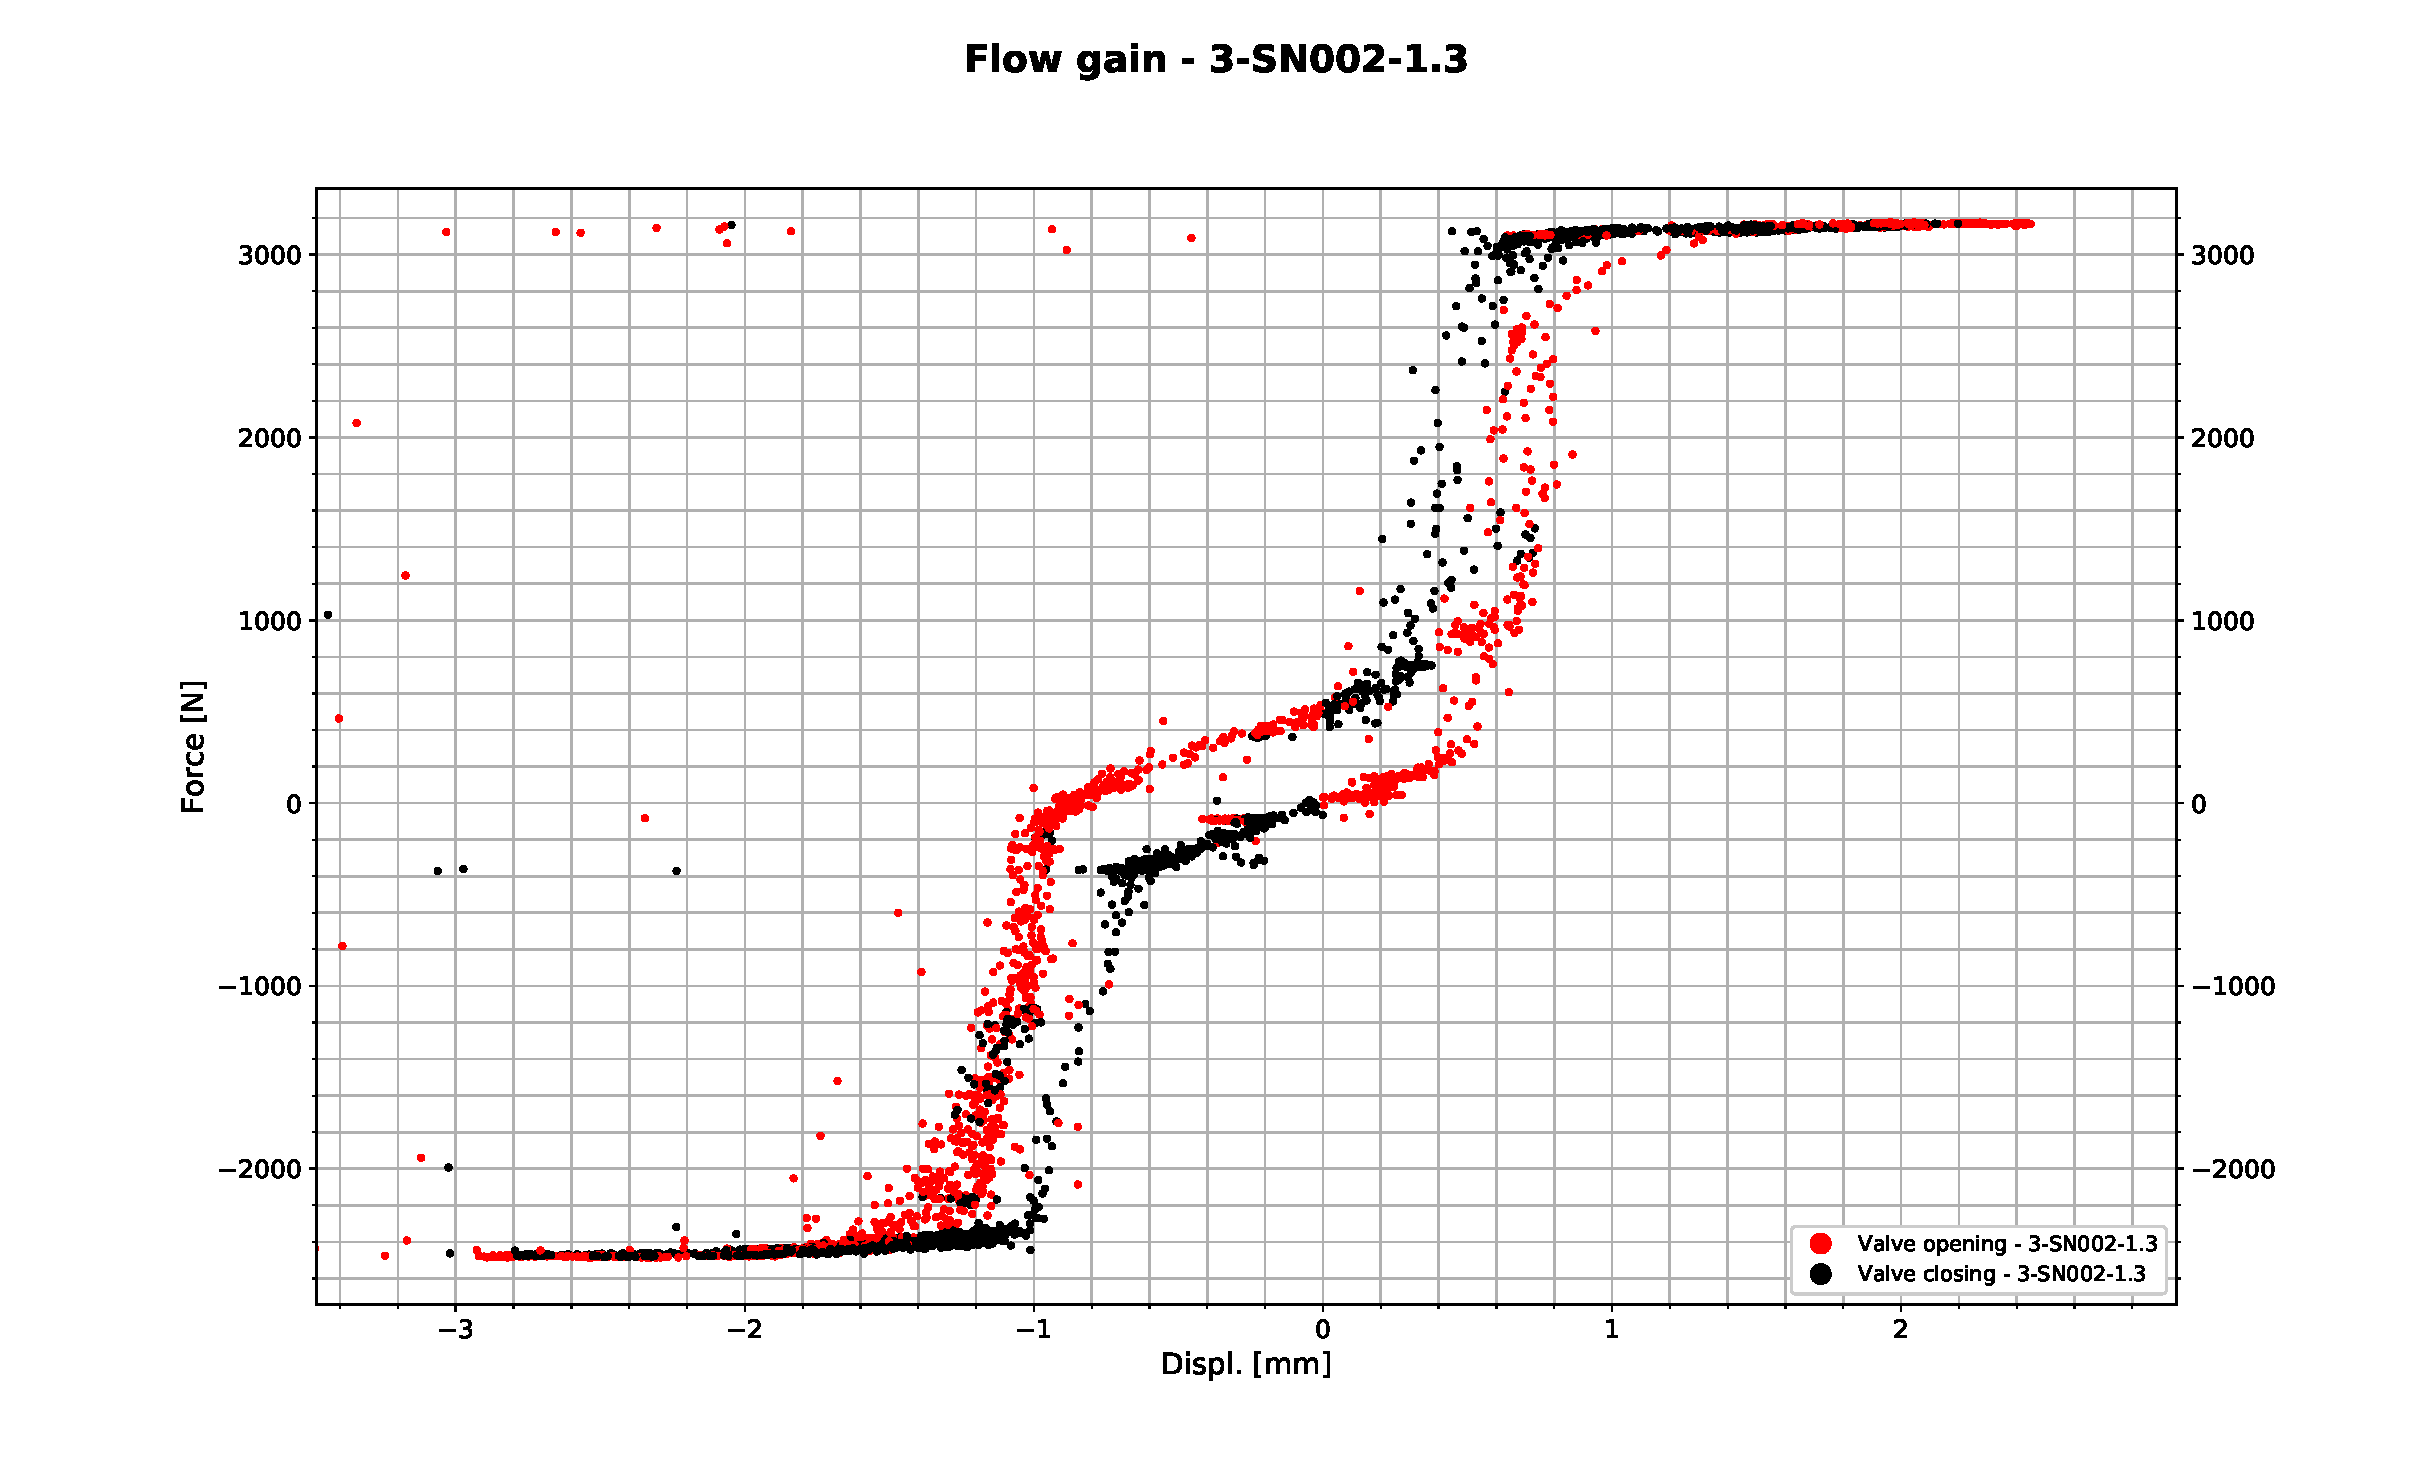
\includegraphics[width=0.9 \textwidth]{figures/flow_gain_example}
      \caption[Force gain curve example]{Force gain curve example. The data correspond to the performed P3 actuators qualification tests.}
      \label{fig:flow_gain_example}
    \end{figure}

  \subsubsection{Kinematic lever model}

    The kinematic relationship between the is governed by the . 
    % Intro, importance of the kinematic model

    These four points and its positioning variables are identified as shown in Figure XX.

    \begin{itemize}
      \item 1: End of the piston rod, center of the piston lug $P_1$
      \item 2: Center of middle circular hole of the input lever $P_2$
      \item 3: Center of circular hole of the input lever at its connection to the pilot input rod $P_3$
      \item 4: Center of circular hole of the input lever at its connection to the piston rod lug $P_4$
    \end{itemize}

    Additionally, these parameters are constant for a considered geometry of the involved components:

    \begin{itemize}
      \item Distance between $P_2$ and $P_4$ -> $l_3$
      \item Distance between $P_2$ and $P_3$ -> $l_1$
      \item Distance between $P_2$ and $P_1$ -> $l_2$
      \item Distance between $P_1$ and $P_4$ -> $l_4$
      \item Angle between the line that connects $P_2$ and $P_3$, and the line that connects $P_2$ and $P_1$ -> $\psi_1$
    \end{itemize}

    The value of $l_1$, $l_2$, $l_3$ and $\psi_1$ are obtained from the geometry of the input lever and the pivoting small lever. Finally, the value of $l_4$ can be obtained as a function of the previously introduced parameters as shown in Equation \ref{eq:l4}.

    \begin{equation}\label{eq:l4}
      l_4 = \sqrt{ (l_1 \sin\psi_1)^2 + (l_2 + l_1 \cos\psi_1)^2 }
    \end{equation}

    %Figure with the labelled points.

    The points movements could be assumed to be in-plane motion, so two coordinates 